\section{Assessments}

\subsection{Quiz Creation}
The Quiz creation page is where a staff member can add questions to a newly created quiz.

\subsubsection{Creating a quiz}
A quiz can be created as a course lecturer or staff member while on a topic group page. That is the intended workflow, however the current implementation is not integrated with the topic group page. A button for adding a new quiz will be visible and once clicked, a modal will appear to initiate the quiz creation:

\begin{figure}[h!]
	\centering
	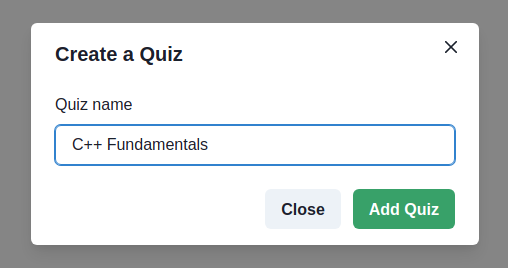
\includegraphics[scale=0.35]{assessments-create-quiz-modal}
	\caption{Quiz creation modal}
\end{figure}

After entering a quiz name and clicking the 'Add Quiz' button, the user will be redirected to the quiz creation page where they can start adding questions.


\begin{figure}[h!]
	\centering
	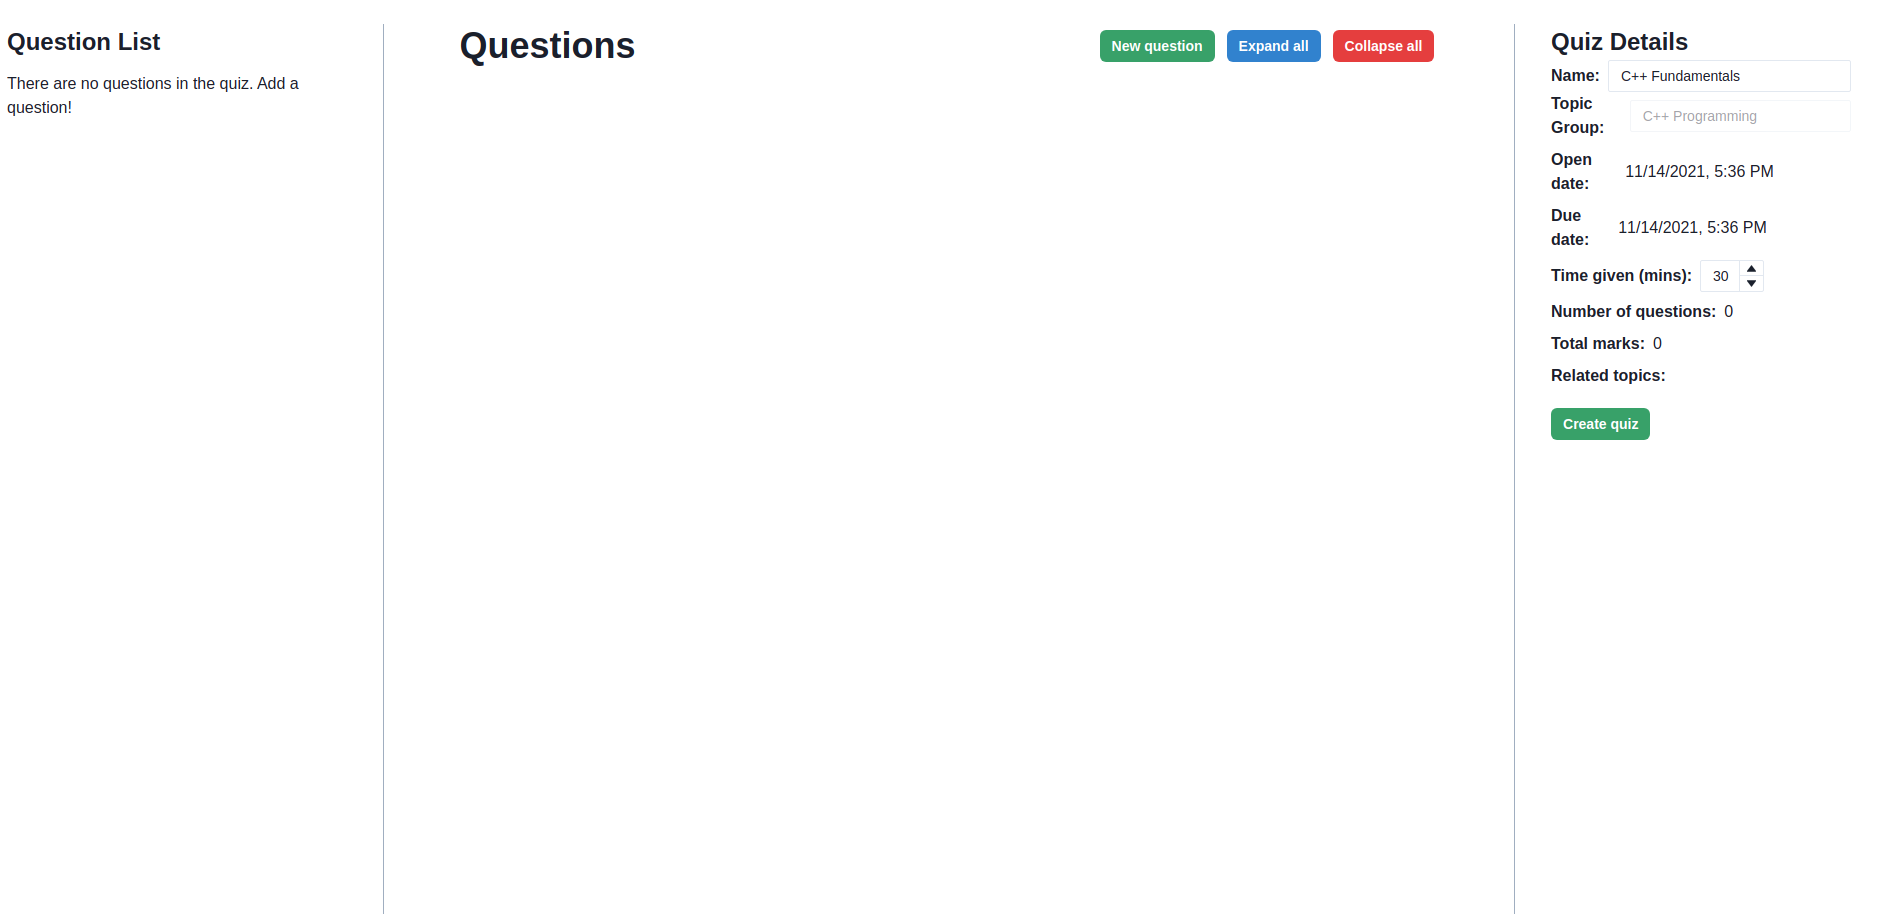
\includegraphics[scale=0.25]{assessments-quiz-creation-interface}
	\caption{Quiz creation page}
\end{figure}


\subsubsection{Adding a question}
To add a question, the user can click on the 'New Question' button.

\begin{figure}[h!]
	\centering
	
\includegraphics[scale=0.35]{assessments-quiz-creation-new-question-button}
	\caption{New Question button}
\end{figure}

A modal will appear, asking the user whether they want to create a new question or import a question that was made and stored in the question bank in a previous quiz. 

\begin{figure}[h!]
	\centering
	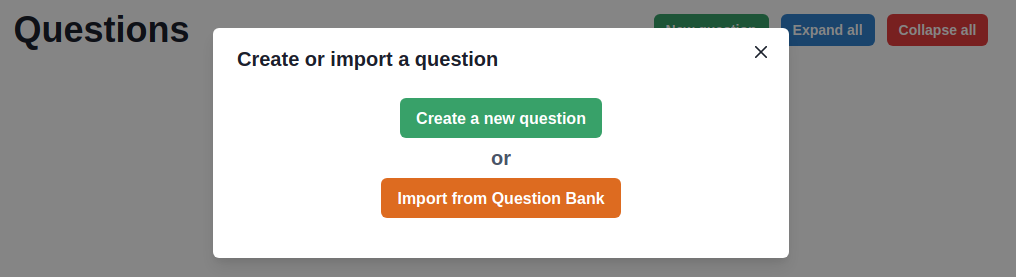
\includegraphics[scale=0.35]{assessments-create-question-modal}
	\caption{Create a question modal}
\end{figure}

Since the import option is incomplete, the user is only able to create a new question as of now. The modal will now update to show data fields for the new question that must be filled in before they're able to add the question to the questions list that was shown on the page. The user can select which topic the question is related to, the question type (multiple choice, short answer and checkboxes) and also add answers along with explanations if desired.

\begin{figure}[h!]
	\centering
	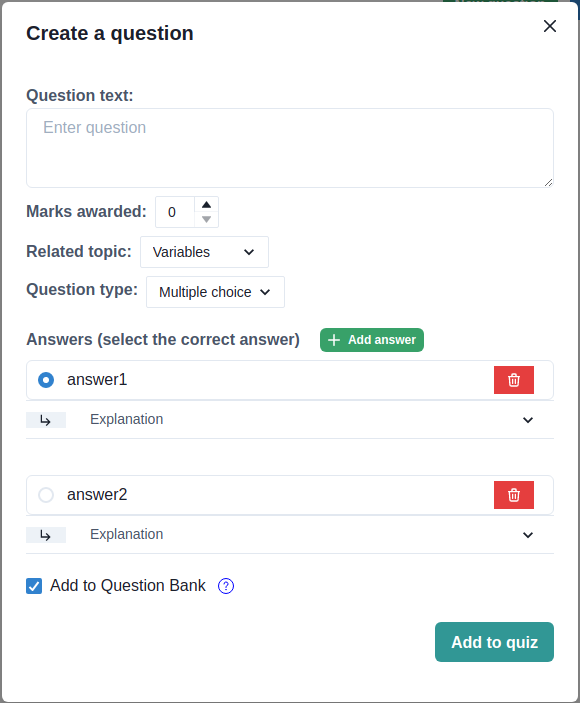
\includegraphics[scale=0.35]{assessments-new-question-modal}
	\caption{New Question data fields}
\end{figure}

The staff member can add an answer via the "Add Answer" button, as well as delete an answer by clicking on the respective red garbage bin icon on a particular answer. Explanations can be added to an answer if desired. An explanation can be added by expanding the 'Explanation' accordion under an answer and entering the explanation there.

\begin{figure}[h!]
	\centering
	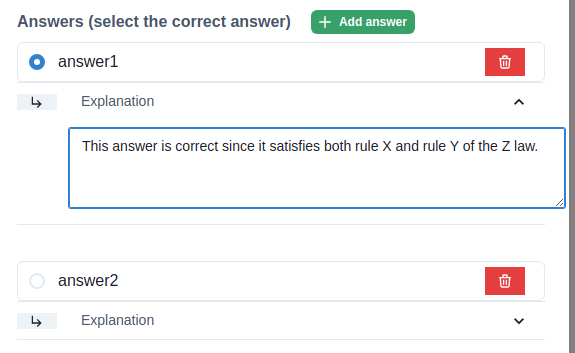
\includegraphics[scale=0.35]{assessments-answer-explanation}
	\caption{Adding an explanation to a possible answer}
\end{figure}

These explanations describe why the specified answer is correct or incorrect, and will be viewable by students who attempted the quiz when they are on the submission review page for the quiz. These allow the staff members to help students understand the topic or concept better with a more detailed explanation than the lecture slides and can also be used as a 'sticky note' with advice by mentioning something like 'revise on Topic X' or 'refer to Lecture Slide X Page Y for a detailed explanation of this concept'. This saves time for the staff member and allows more immediate help for the students instead of them asking a question on the forums.

Once the fields have been filled in, the staff member clicks on the "Add to Quiz" button to add the question to the questions section. By default, "Add to Question Bank" is ticked so all questions will automatically be saved in the question bank for future re-use.

\begin{figure}[h!]
	\centering
	
\includegraphics[scale=0.35]{assessments-add-to-quiz-button}
	\caption{Add To Quiz button}
\end{figure}

The question will appear in the question list and questions section. The question list displays the marks awarded and topic for each question and allows the staff member to quickly see whether they need to add more questions, keep track of marks for each question, and whether to add more or less questions for a particular topic. In the quiz details, the number of questions for a topic is also shown. In the below image, there is 1 question for the topic "Variables".

\begin{figure}[!hbpt]
	\centering
	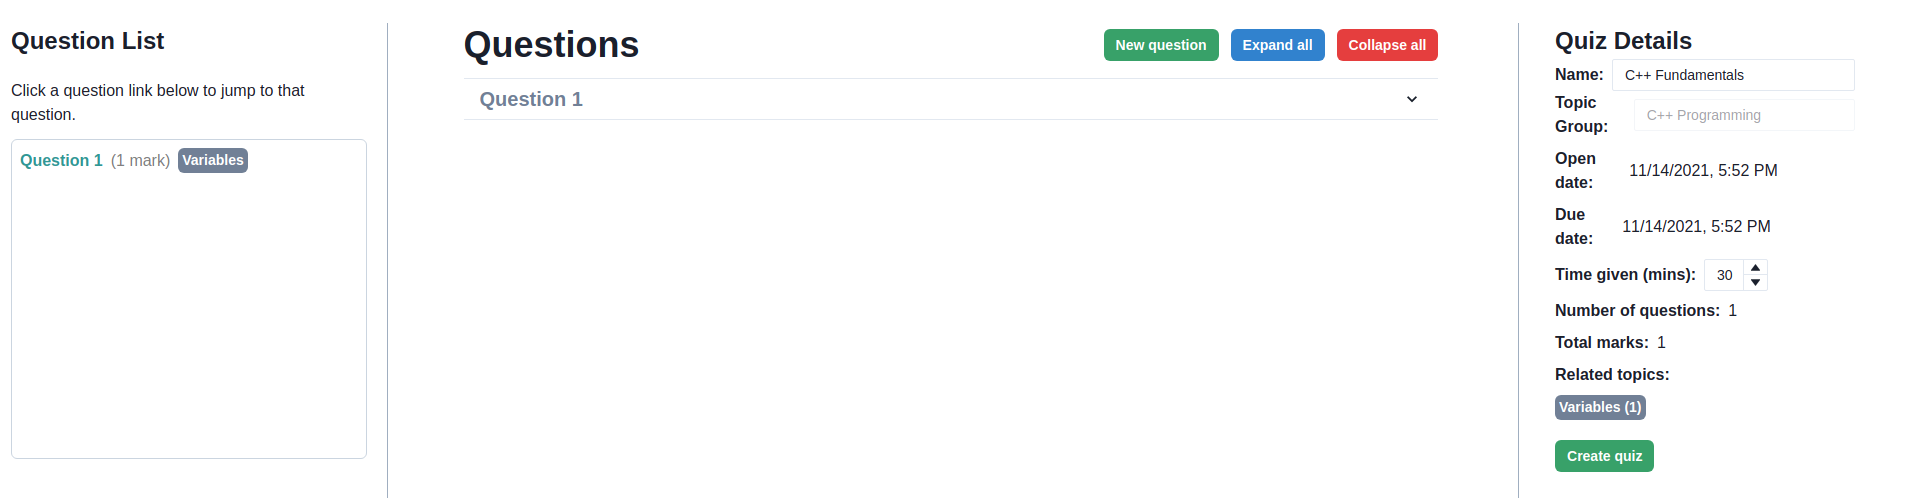
\includegraphics[scale=0.25]{assessments-question-list}
	\caption{Question list and section}
\end{figure}

To show fields of a particular question, you can expand it by clicking on its header in the question section, or on its question list link. Similarly, you can collapse a question by clicking on a question's header/link while it's expanded. There is also a "Expand all" and "Collapse All" button to expand or collapse all questions.

\begin{figure}[h!]
	\centering
	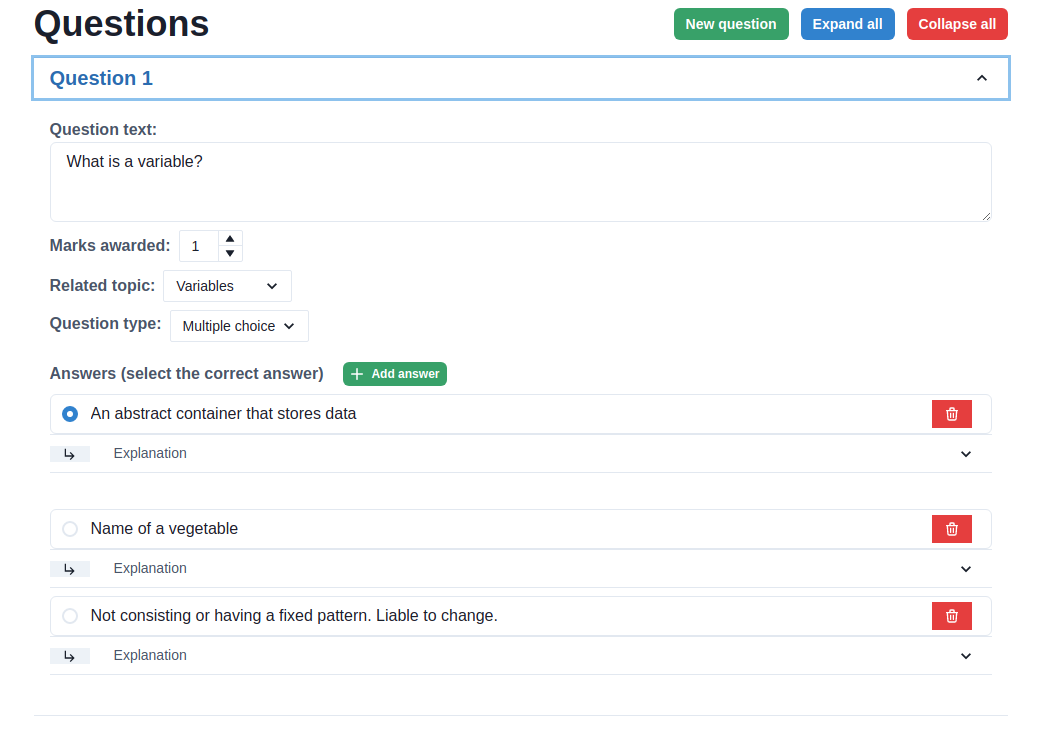
\includegraphics[scale=0.35]{assessments-expand-question}
	\caption{Question list and section}
\end{figure}


\subsubsection{Editing quiz details}
The quiz name, open date, due date and time given can be modified in the Quiz Details column of the Quiz Creation page. Other details such as the number of questions and total marks are displayed. 

\begin{figure}[h!]
	\centering
	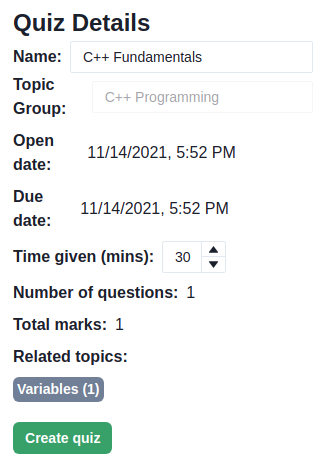
\includegraphics[scale=0.35]{assessments-quiz-details}
	\caption{Quiz details}
\end{figure}


\subsection{Quiz Usage}
The Quiz Usage page is where students enrolled in a topic group can attempt a quiz that was made for the topic group. From left to right, the columns are the quiz progression column, the question itself, and the timer showing the time remaining for the quiz attempt. The quiz progression column indicates to the student which questions they've attempted or not attempted yet. A blue icon with a question mark represents an unattempted question while a green icon with a tick represents an attempted question. This allows the student to be always aware of which questions they'll need to go back to later. The student can also click on any of the question number icons to jump to that particular question. 

\begin{figure}[h!]
	\centering
	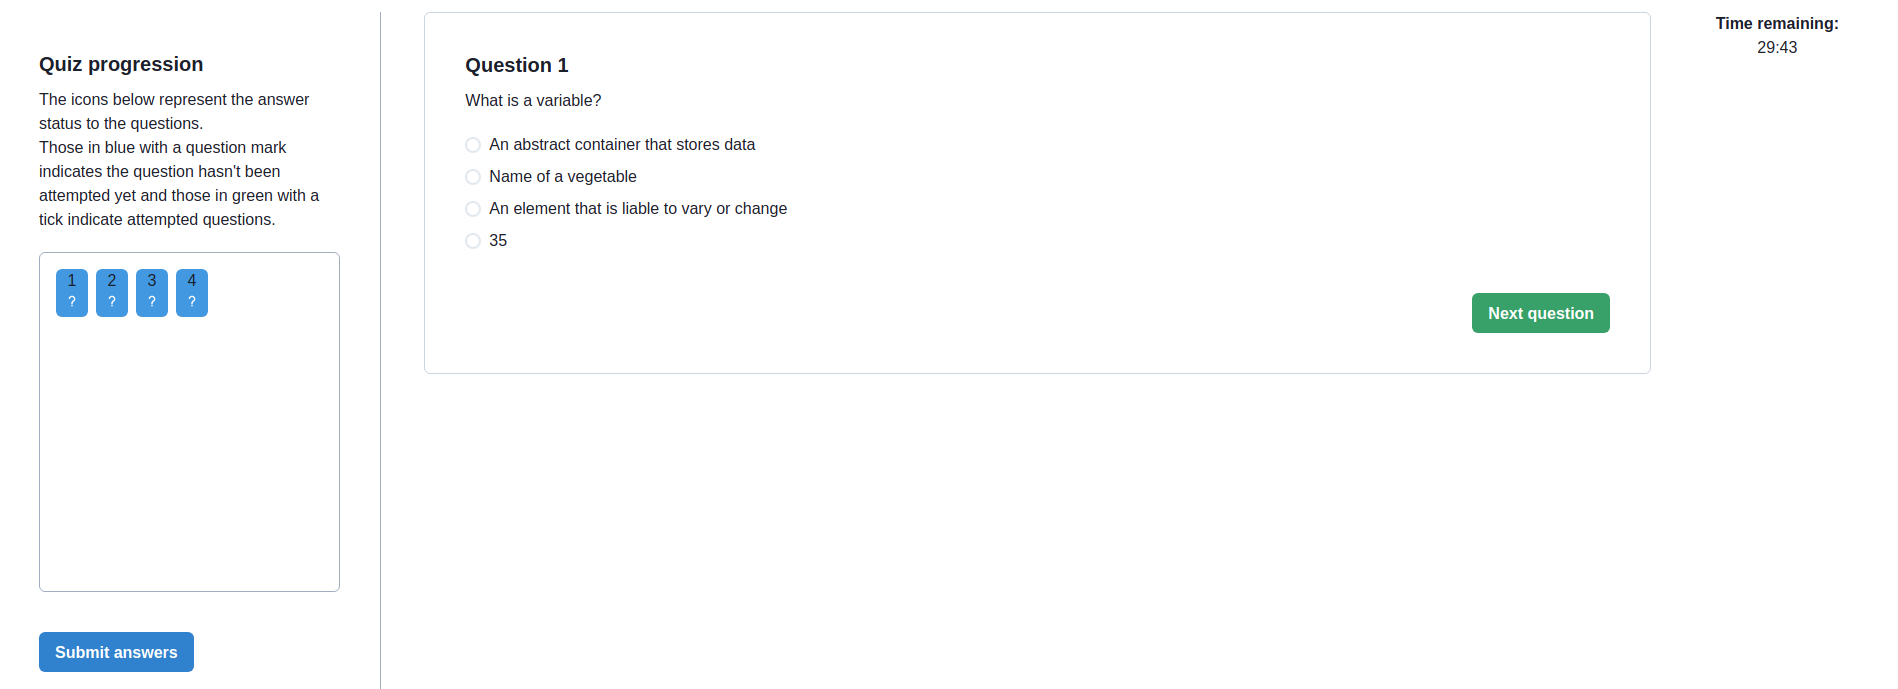
\includegraphics[scale=0.25]{assessments-quiz-submission}
	\caption{Quiz submission page}
\end{figure}

\subsubsection{Answering a question}
The student can answer a question by clicking on one of the options (multiple choice), one or more of the options (checkbox), or by entering text into the textbox (short answer). 

Once they've selected an answer, that counts as an attempt of the question and the question icon (in the quiz progression column) for that question will turn green with a tick as shown below.

\begin{figure}[h!]
	\centering
	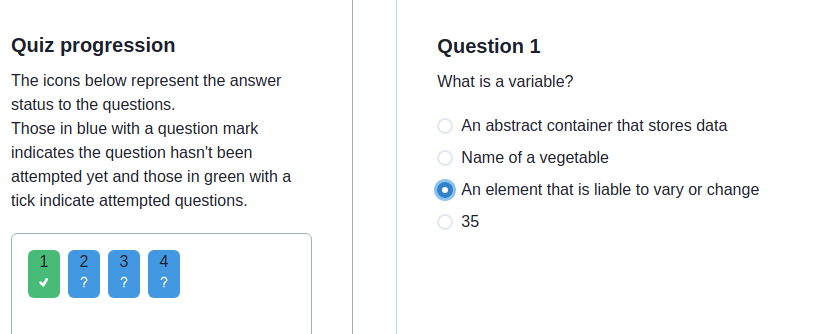
\includegraphics[scale=0.35]{assessments-question-attempt}
	\caption{Successful question attempt}
\end{figure}


\subsubsection{Editing an answer}
To edit an answer, the student can select another possible answer and their new answer will be the updated answer to the question.

\begin{figure}[h!]
	\centering
	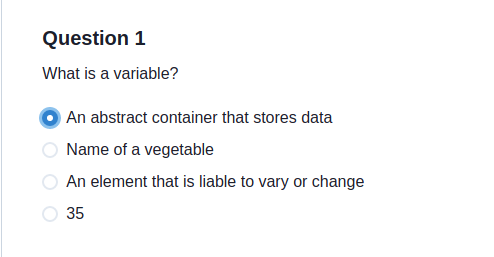
\includegraphics[scale=0.35]{assessments-editing-answer}
	\caption{Editing an answer}
\end{figure}


\subsubsection{Submitting an attempt}
Once the student is satisfied with their submission, they can click on the "Submit answer" button below the Quiz Progression section to submit their quiz submission.

\begin{figure}[h!]
	\centering
	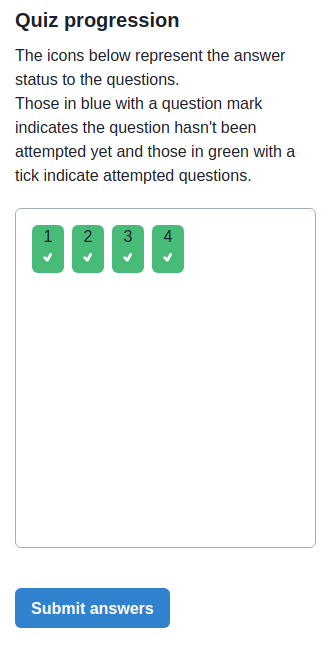
\includegraphics[scale=0.35]{assessments-submit-answers-button}
	\caption{Submitting answers button}
\end{figure}

A confirmation modal will appear before the quiz submission is submitted and no changes can no longer be made to the attempt.

\begin{figure}[h!]
	\centering
	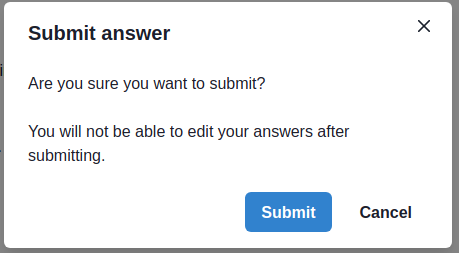
\includegraphics[scale=0.35]{assessments-submit-attempt-modal}
	\caption{Submit quiz attempt confirmation modal}
\end{figure}

After pressing the "Submit" button, a submission confirmation message will be shown.

\begin{figure}[h!]
	\centering
	
\includegraphics[scale=0.35]{assessments-successful-quiz-submission-message}
	\caption{Successful quiz submission message}
\end{figure}


\subsection{Viewing quiz results and feedback}
After a student has submitted their quiz attempt, their attempt has been marked and the due date has passed, the student can review their quiz submission on the Quiz Review Submission page.

\begin{figure}[h!]
	\centering
	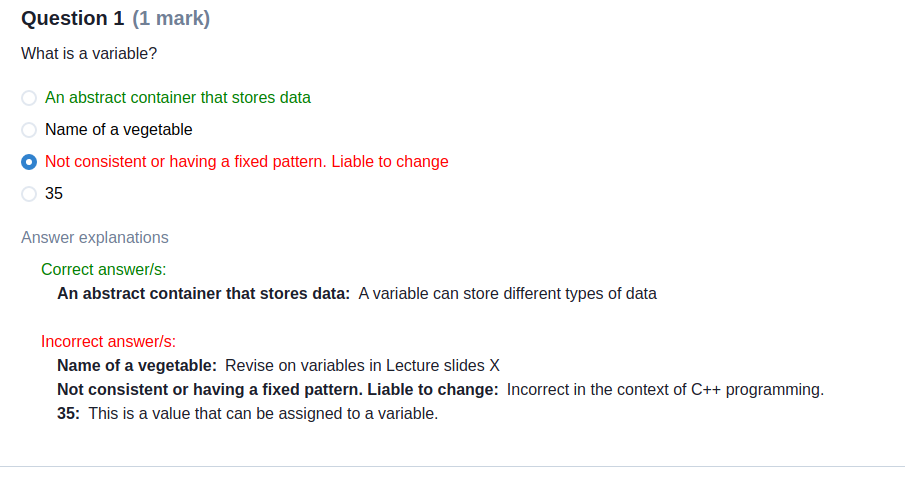
\includegraphics[scale=0.35]{assessments-view-submission}
	\caption{Review submission page}
\end{figure}

\subsubsection{Viewing correct answers against their answers}
The student can compare their answers with the correct answers. If they answered a question incorrectly, their selected answer's text will turn red and the correct answer's text will turn green.

\begin{figure}[h!]
	\centering
	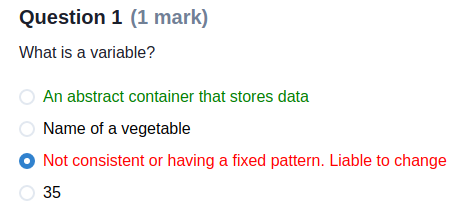
\includegraphics[scale=0.35]{assessments-compare-answers}
	\caption{Compare correct answers against a student's answers}
\end{figure}


\subsubsection{Viewing an explanation of the correct answer and incorrect answers}
Below the possible answers will be the explanations, if the staff member has written any. Explanations for all the answers will be shown. This allows the student to understand why a particular answer is wrong or right.

\begin{figure}[h!]
	\centering
	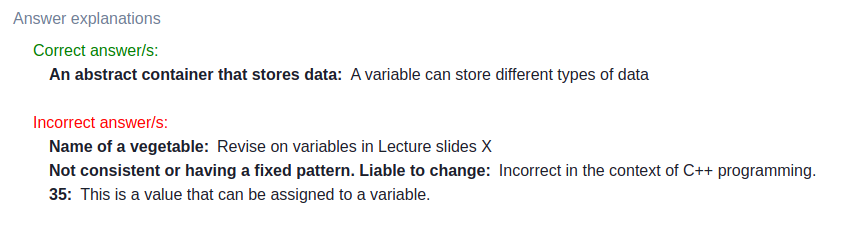
\includegraphics[scale=0.35]{assessments-view-explanations}
	\caption{View explanations for each answer to a question (if provided)}
\end{figure}


\subsection{User Interface Design}
The user interface is what the user relies on to complete tasks and thus it is important that the design is usable and easy to use. A few changes were made from the initial designs to support the added content that was not planned in earlier stages of the Assessments feature.

\subsubsection{Final Designs}
The final design had more emphasis on possible tools that'd improve the user experience and was added to reduce the amount of time the user needs to spend on their tasks: 

\begin{enumerate}
	\item Quiz Creation page: contains the questions list and the expand/collapse functionality to allow the user to focus on particular questions
	\item Quiz Usage page: contains the quiz progression column that allows them to keep track of which questions they've attempted or not attempted as well as the ability to navigate to any question with one click
	\item Quiz Review Submission page: highlights incorrect answers vs. the correct answers and shows all explanations (that were provided by the quiz creator) for the possible answers
\end{enumerate}

\begin{figure}[h!]
	\centering
	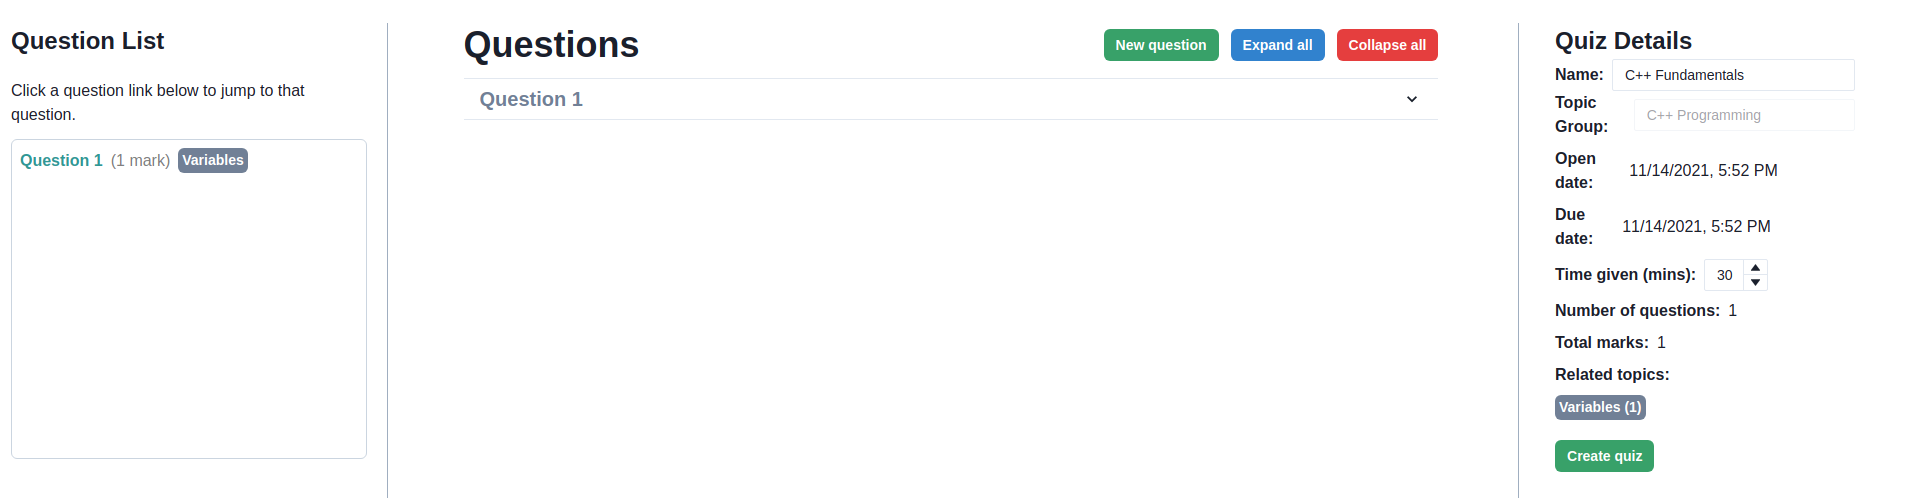
\includegraphics[scale=0.35]{assessments-question-list}
	\caption{Quiz creation page}
\end{figure}

\begin{figure}[h!]
	\centering
	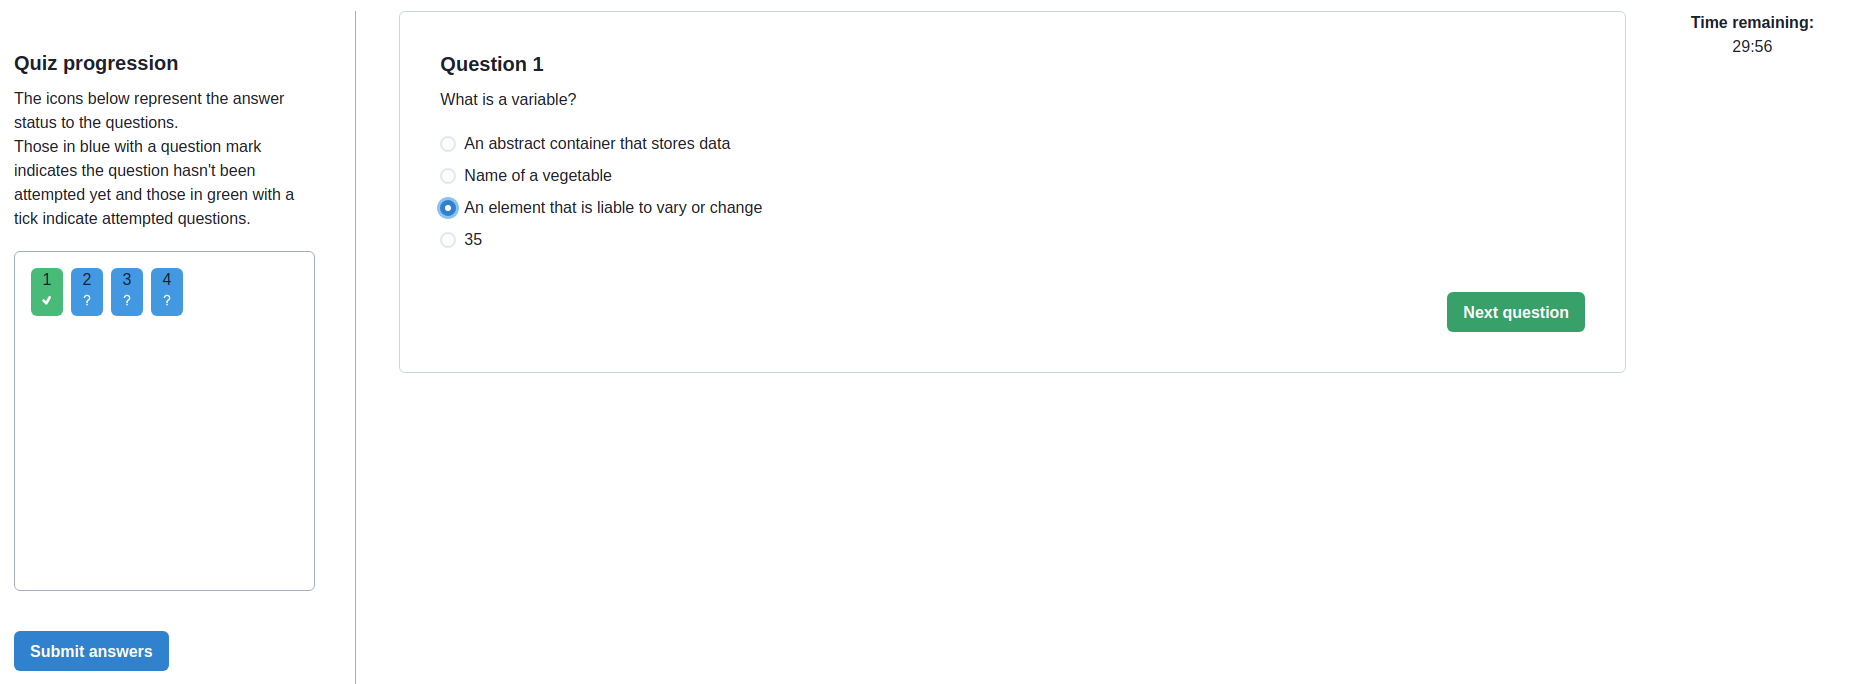
\includegraphics[scale=0.35]{assessments-quiz-usage-interface}
	\caption{Quiz usage page}
\end{figure}

\begin{figure}[h!]
	\centering
	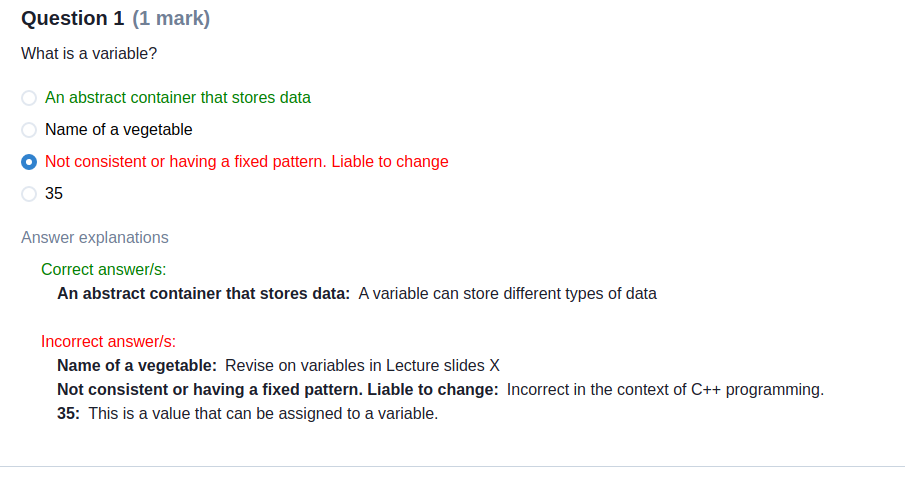
\includegraphics[scale=0.35]{assessments-view-submission}
	\caption{Quiz review submission page}
\end{figure}


\subsubsection{Changes Made From Initial Designs}
There were significant changes to the initial designs in terms of button layouts and colour schemes, however the core content displayed is the same. Additional data that was not foreseen or thought of during initial designing was added to the user interface design. Furthermore, extra tools were added for convenience and to improve the user experience. 

Below, the initial and final designs next to each other to see the similarities and differences.

\newpage
Question creation:

\begin{figure}[h!]
	\centering
	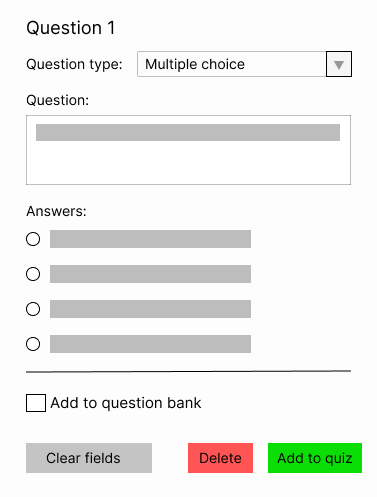
\includegraphics[scale=0.35]{assessments-quiz-creation}
	\caption{Initial design of question creation}
\end{figure}

\begin{figure}[h!]
	\centering
	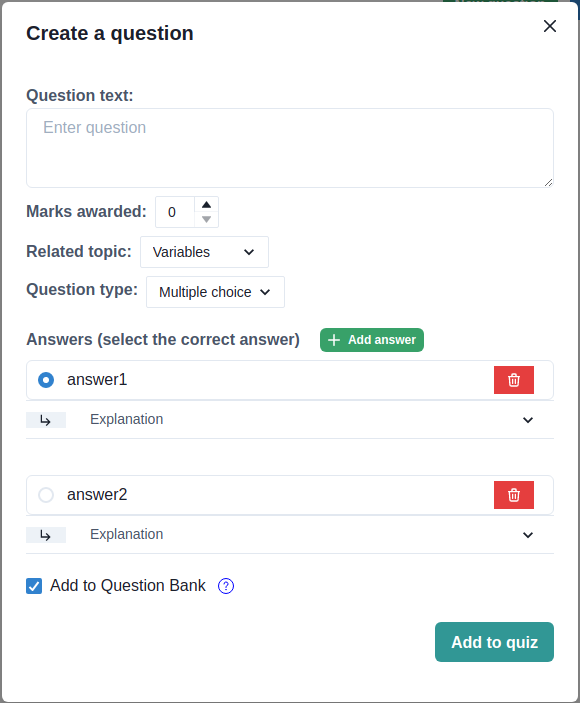
\includegraphics[scale=0.35]{assessments-new-question-modal}
	\caption{Final design of question creation}
\end{figure}

\newpage

Quiz usage:

\begin{figure}[h!]
	\centering
	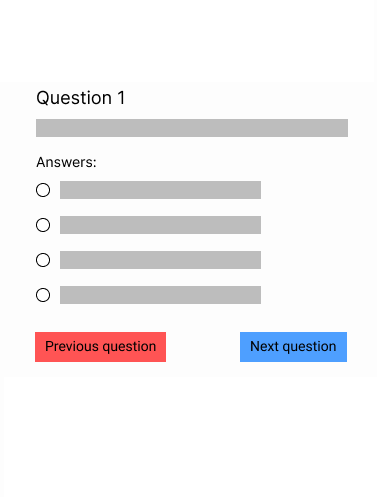
\includegraphics[scale=0.35]{assessments-quiz-usage}
	\caption{Initial design of quiz usage}
\end{figure}

\begin{figure}[h!]
	\centering
	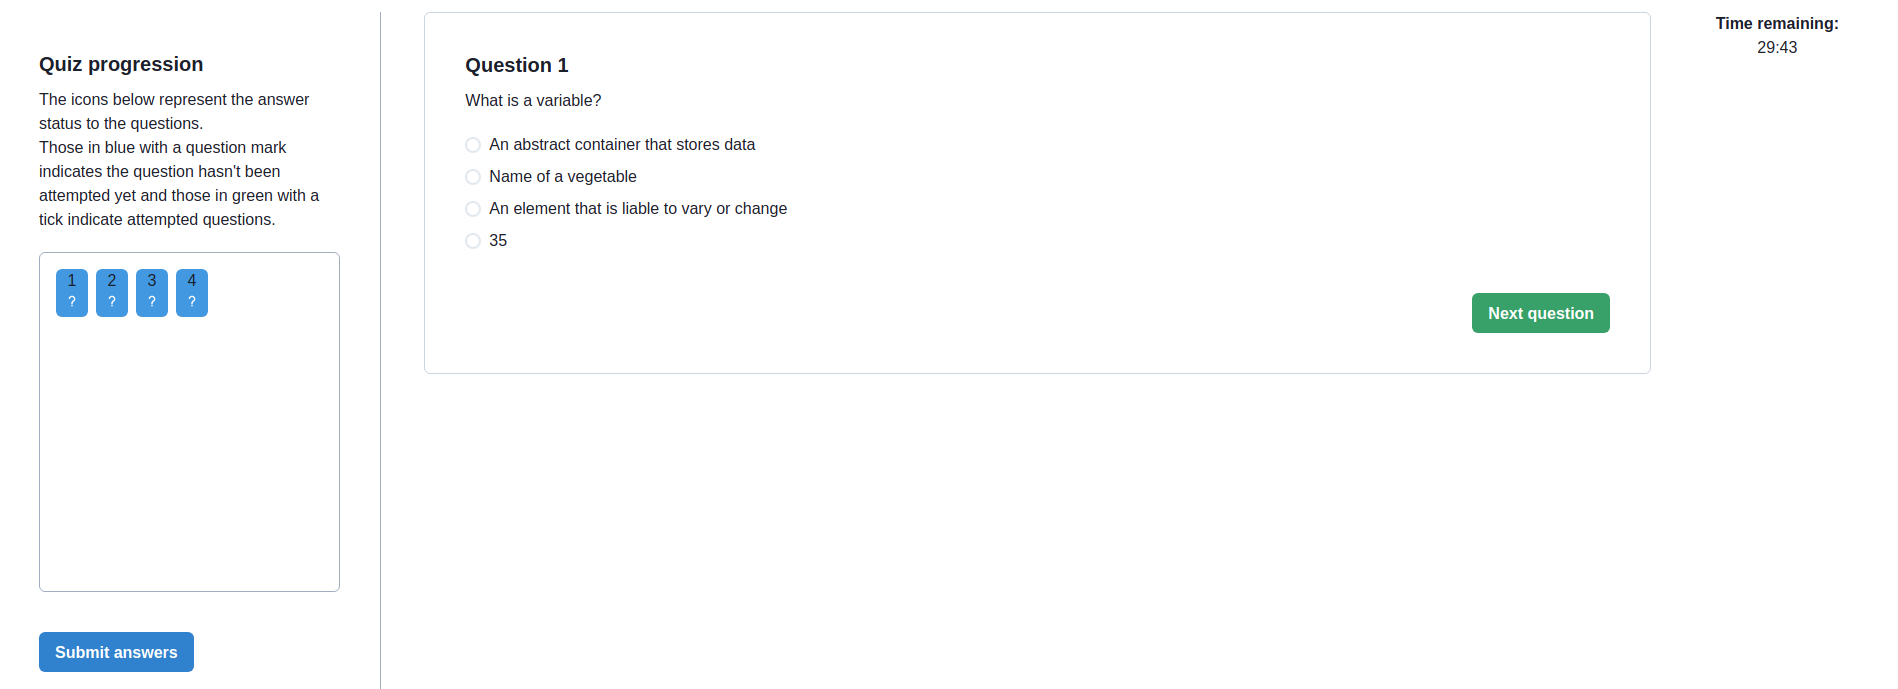
\includegraphics[scale=0.25]{assessments-quiz-submission}
	\caption{Final design of quiz usage}
\end{figure}

\newpage